\documentclass{article}
\usepackage{preamble}

\title{Thesis Preparation Report}
\author{Jonas Tonny Nielsen \and Jonas Lomholdt}
\date{\today}

\begin{document}

\maketitle

\listoftodos

\tableofcontents
\listoffigures
%\listoftables

\todo{Hand-in Jan 8th or 11th}

\section{Introduction} % Introduction to the project
A number of studies have shown that introducing clicker systems, also known as Classroom Response Systems (CRS), into classrooms has a positive effect on learning outcomes and classroom interactivity \cite{yourstone2008classroom, siau2006use, lantz2014effectiveness}. 

The idea of a CRS is not a new one and low-tech versions have been used in classrooms before, where students simply hold up a piece of paper, called a response card, with their answers \cite{ralph1994effects}. 
Later more modern versions are introduced, the so called \emph{clickers}. A clicker is a device, that allows users (and in many cases, students) to respond to questions in a classroom environment. These systems are defined by \citeA{lantz2014effectiveness} in it's most common form as 

\begin{quote}
    \emph{"[...] individual response devices held by individual students allowing them to quickly and anonymously respond to multiple choice questions presented in class. A receiver attached to a classroom computer collects and summarizes the responses instantly and projects them graphically onto the screen for students and the educator to see"} \cite{lantz2014effectiveness}
\end{quote}

As described above, the clicker itself is used for collecting answers from the students via a clicker device. Many different versions exists, and one example can be seen in figure \ref{fig:iclicker} below. The device connects to a receiver in the classroom and the receiver is then again connected to a computer that stores and displays the data through a piece of software.

\begin{figure}[H]
\capstart
	\centering
		\frame{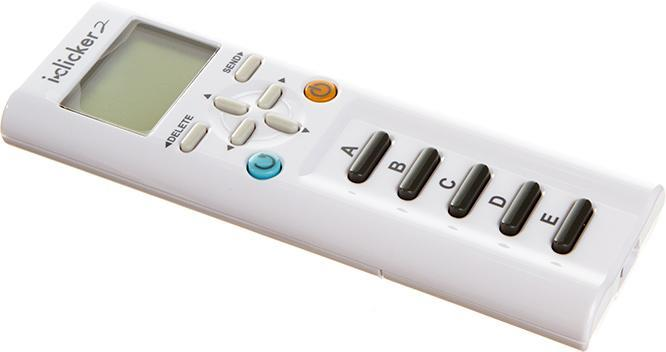
\includegraphics[width=\textwidth]{iclicker.jpg}}
        %\missingfigure{iClicker - An example of an iClicker}
	\caption[iClicker2]{One example of a clicker device called the iClicker2 \label{fig:iclicker}}
\end{figure}

A regular CRS like the one mentioned above is very common, but does introduce a variety of pros and cons. This includes the investment in the clicker devices and the potential issues of setting up the receiver and more. With the emerging of smartphones and fast, reliable internet connections, it would seem plausible to use devices that the users already have, effectively swapping out the clicker device with a smartphone or a laptop. The concept is known as Bring Your Own Device or \emph{BYOD} \cite<Johnson et al., 2013 in>[p.~329]{stowell2015use}. This has indeed been implemented with mixed results (as we will describe in the following section), and introduces a whole new range of possibilities and challenges. 


There are examples of CRS systems available online, and all takes a different approach. Some are made exclusively for children or ground-schoolers (e.g., \url{https://kahoot.it}), and some are feature rich, made for conferences and classrooms (e.g., \url{http://socrative.com}, \url{https://www.polleverywhere.com} and \url{https://www.iclicker.com/}). The most appealing and well implemented version we could find was Mentimeter (\url{https://www.mentimeter.com}), which supports many of the features that would be expected of a fully functional CRS. Most of the existing literature about CRS is centered around physical clickers and the learning outcomes/improvements of using them, though there seems to be a lack of research of the use of such systems within the last few years, where smartphones has become widespread and popular among students \cite[p.~329]{stowell2015use}.


As mentioned above, the obvious approach would be to leverage the technology that students already use. In the case of the IT University of Copenhagen (ITU), laptops are mandatory and a internet connection is provided by the university, so the hardware aspect is already in place. We will implement CRS software that is capable of asking technical (and non-technical) questions as described above on both mobile and laptops alike.



%%% explain a poll, and 'polling' and 'polling devices'
%%% explain polling fatigue


%\cite{yourstone2008classroom}

\section{Literature Review} % What is already known and done + existing solutions?

%%% Some intro to this maybe...

Some of the least resent literature dating back to around 2007, is mainly focused on physical clicker devices, where the students buy actual "remote controls" for polling, in a time where more modern solutions (including the smartphone) has not yet matured. And even today, the physical clicker devices still seem to play a significant role in the \emph{"clicker community"}. \citeA{stowell2015use} explains how the use of clicker systems on physical devices has a greater response rate compared to mobile, but with no significant differences in the final grades. Also the introduction of students bringing their own devices (the so called \emph{Bring Your Own Device}) introduces new issues such as internet connectivity and the risk of being distracted by the device itself (pp. 331-332).


One of the main reasons to use a CRS is the importance of interactivity in learning \cite{draper2004increasing}. Studies find that CRS engages interactivity, helps students stay active during lectures \cite[p.~116]{moredich2007engaging}, improves learning \cite<e.g.,>{siau2006use, yourstone2008classroom} and increases attention \cite[pp.~86-88]{sun2014influence}. While \citeA{yourstone2008classroom} focuses on actual results in learning outcomes and \citeA{sun2014influence} uses brainwave analysis to determine level of attention while using CRS, most other studies take on a qualitative approach and evaluate teachers and students by asking to their engagement, participation and learning outcomes \cite<e.g.,>{moredich2007engaging}. The latter approach seems to be the most widespread in the literature and focuses more on whether or not students feel an increased engagement and participation rather than their actual performance and examination results. 


\citeA{stowell2007benefits} takes on the qualitative approach where they ask into students emotions towards an introductory psychology class before, during and after lecture. The study compares standard lectures to hand raising, response card and "clicker" lectures\footnote{Standard lectures are thought of as normal lectures where the teacher asks open ended questions to the students. Hand raising is the approach where students are asked to raise their hand if they agree to a statement. Response cards are cards labeled A, B, C, D and are sort of the same as hand raising \cite[p.~254]{stowell2007benefits}.}.
They find that more correct answers to questions are present in response card lectures but explains the much higher correctness with the ability to see what peers are answering \cite[p.~257]{stowell2007benefits}. The same applies for hand raising. Furthermore the study finds that there's a small positive impact on emotions towards the class depending on which kind of lecture is taught (i.e. standard, hand raising, response card and "clicker"). \cite{stowell2007benefits}.


Among the biggest studies of CRS is \emph{Increasing interactivity in lectures using an electronic voting system} by \citeA{draper2004increasing}. This particular study took place over a two year period and found (among other things) that the benefits increases as teachers became aware how to exploit the pedagogy behind the system \cite[p.~93]{draper2004increasing}. The study took place in a time where there was a need for physical hardware (e.g., remote controllers and receivers) in order to facilitate a CRS. This study addresses the need to learn how to proper use a CRS in order to get the benefits from it.









%\section{Method}





\section{Detailed future plan} %\todo{New headline?}



% Reason about the tools to be used in the project
% Design the system based on the structure mentioned below
% Implement the system, and launch to a website
% Create questionnaire for in-class research
% Complete questionnaire in classroom // without CRS system
% Complete questionnaire in classroom // with CRS system
% Figure out if the CRS system engages students more
% Finish report





%%% Questions to Peter
    % Should the questionnaire be general for both non and clicker questions? Or should there be two different ones?
    
    
    % I feel I'm participating in the lecture.
    % I feel confident raising my hand in lectures.
    % I feel I contribute with my opinion.
    % It's easy to avoid participating in lectures.
    % Students interact with the instructor in class. Students are involved in learning during class. Students are engaged in class.
    Students are attentive in class.
    Students participate in class discussion.
    Students provide their opinions to questions from the in- structor during the class.
    Students receive feedback in class on their understanding of the course materials.
    Students receive feedback from the instructor during the class.
    Students can gauge whether they are following the course materials during the class.
    Students can assess their understanding of the course ma- terials with respect to other students during the class.

    I interact with the instructor in class. 2. I am involved in learning during class. 3. I am engaged in class.
    4. I am attentive in class.
    I participate in class discussion.
    I provide my opinion to questions from the instructor during the class.
    I receive feedback in class on my understanding of the course materials.
    I receive feedback from the instructor during the class.
    I can gauge whether I am following the course materials during the class.
    I can assess my understanding of the course materials with respect to other students during the class.
    
    %%% CRS
    % I feel more confident about the material taught in class
    % I would recommend using a CRS in other classes 
    % I feel more confident answering questions through a CRS than by hand raising
    % I participate more in class while using a CRS
    % I would feel more confident going to an exam using a CRS in class than not doing it
    % I'm more engaged during classes while using a CRS
    % I like to get feedback and answers to questions immediately
    
    
    % I feel more distracted by using a CRS in class
    % 


We want to develop a classroom response system from scratch. The system should include features that support asking and answering technical questions. 
%%% We should be able to display code, including linenumbers and syntax highlighting!

In order to use the system, a user needs to register and log in. When logged in the user is presented with a dashboard from where it's possible to see which rooms a user is a member of or administrating. Every user is able to create and administer rooms from where it's possible to create questions. A flow diagram of this process is shown in figure \ref{fig:flow-diagram} 

\begin{figure}[H]
    \capstart
	\centering
	\smartdiagramset{
        back arrow disabled = true,
        uniform color list=gray!60!black for 5 items
    }
    
    \smartdiagram[flow diagram:horizontal]
    {Register, Log In, User Dashboard, Room, Questions}
    
	\caption[Flow Diagram]{A flow diagram of the core features \label{fig:flow-diagram}}
\end{figure}

It should be possible to search for and sign up to rooms from the dashboard. Within a room, questions are created and published by the administrator and as questions are published and made available, members of the room should be able to answer the questions. This way, the questioner can prepare a series of questions related to a lecture, and only make the questions available when he/she wants to receive answers. Information about a new available question should be pushed to online members of the room. A number on the questioners screen should tell how many members have answered the question. When the questioner choose to close a question and thereby stop receiving answers, the results should be presented in a style chosen by the questioner. The questioner can mark an answer as correct if there's single correct answer to a question. It should be possible for all members of a room to go back and look at previous available questions.

The system should support asking questions with included code and the system should be able to present it in a nice and readable way. Code should be presented and formatted with indentions, line numbers and syntax highlighting just like any text editor or IDE would do it. The purpose is to be able to ask questions which could be relevant to ask students who are taking classes related to software development.





%\subsection{Possible implementation thoughts}

%\subsection{Features} % The features of the system

%Users
    %user roles
        %Admin
        %Teacher
        %Student
    %Profile picture
%Classrooms
    %Search for classrooms
    %Create classroom (teachers only)
    %Invite students to classrooms
    %Group questions by tags
    %Invite to classroom by email
    %Request access to classroom
    %Delete classrooms
%Questions
    %Create questions of different types (teachers only)
        %Multiple Choice questions
        %Include pictures
        %Fill-in-the-blank questions
    %Questions should be open and closeable by teachers (students can/cannot answer)
    %Students should be notified when new questions are available
    %Questions should be publishable
    %Delete questions
    %Add tags/labels
%Dashboard (teacher)
    %Graphs with answer overview
    %Real-time feed of answers (Pusher/Sockets, green check mark if answered red cross if not-ish)
%Dashboard (student)
    %See classrooms
    %See question history


% RESTfull service 
% thesis.com/classroom/advanced-programming-2015/question/16/

\subsection{Database design} \todo{Write this section.}


\begin{figure}[H]
\capstart
	\centering
		%\includegraphics[scale=0.65]{ClassHTMLList.png}
        \missingfigure{Database Design}
	\caption{Database Design\label{fig:database-design}}
\end{figure}






%--------------------REFERENCES--------------------%
\bibliographystyle{apacite}
\bibliography{ref.bib}


\end{document}
